\subsection{Favorieten}\label{favorieten}
Op het \emph{Intranet} is een favorieten functionaliteit beschikbaar. Aan de onderkant van elke content pagina vind je een link, genaamd \emph{Toevoegen aan favorieten} of \emph{Verwijderen uit favorieten}. Met deze twee links kun je de pagina toevoegen aan of verwijderen uit de favorieten lijst.

De onderstaande afbeelding toont hoe een lijstje met favorieten eruit ziet.

\begin{center}
	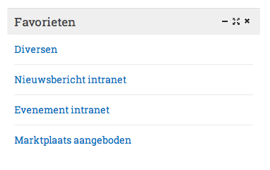
\includegraphics[width=\textwidth]{img/favorieten1}
\end{center}

De onderstaande afbeelding toont de link waarmee je een content pagina kan toevoegen aan favorieten.

\begin{center}
	
\includegraphics[width=\textwidth]{img/favorieten2}
\end{center}

De onderstaande afbeelding toont de link waarmee je een content pagina kan verwijderen uit favorieten.

\begin{center}
	
\includegraphics[width=\textwidth]{img/favorieten3}
\end{center}